\chapter{Programowanie dynamiczne}

\makeatletter
\def\input@path{{chapter15/}}
\makeatother

\subchapter{Planowanie czynności na liniach montażowych}

\exercise %15.1-1
Poniższa rekurencyjna procedura wypisuje wszystkie stanowiska o~numerach od 1 do $j$ w~kolejności rosnącej, przy założeniu, że linia użyta na stanowisku $j$ ma numer $i$.
Do wywołania rekurencyjnego przekazywany jest numer wykorzystanej linii na stanowisku $j-1$ odczytany z~$l_i[j]$.
Imitowane jest dzięki temu zachowanie pętli z~oryginalnej procedury.
\begin{codebox}
\Procname{$\proc{Print-Stations}'(l,i,j)$}
\li	\If $j\ge1$
\li	\Then $\proc{Print-Stations}'(l,l_i[j],j-1)$
\li		wypisz ,,linia '' $i$ ,,{}, stanowisko '' $j$
	\End
\end{codebox}
Aby wypisać cały ciąg stanowisk, należy wywołać $\proc{Print-Stations}'(l,l^*\!,n)$.

\exercise %15.1-2
W~pierwszym kroku indukcyjnym wzór oczywiście zachodzi:
\[
	r_1(n) = r_2(n) = 1 = 2^{n-n}.
\]
Niech teraz $j=1$, 2, \dots, $n-1$ i~przyjmijmy, że $r_1(j+1)=r_2(j+1)=2^{n-(j+1)}$.
Stąd
\[
	r_1(j) = r_2(j) = r_1(j+1)+r_2(j+1) = 2^{n-(j+1)}+2^{n-(j+1)} = 2^{n-(j+1)+1} = 2^{n-j},
\]
a~więc wzór jest prawdziwy dla dowolnego $j$.

\exercise %15.1-3
Na podstawie wyniku poprzedniego zadania oraz wzoru (A.5), łączna liczba odwołań do wartości $f_i[j]$ wynosi:
\[
	\sum_{i=1}^2\sum_{j=1}^nr_i(j) = 2\sum_{j=1}^n2^{n-j} = 2\sum_{k=0}^{n-1}2^k = 2\cdot\frac{2^n-1}{2-1} = 2^{n+1}-2.
\]

\exercise %15.1-4
Możemy zrezygnować z~większości komórek tablic $f_i$.
Wystarczy zauważyć, że jedynymi wartościami z~tablic $f_i$ potrzebnymi do obliczenia $f_i[j]$ są $f_i[j-1]$.
Tablice $f_i$ nie są też wykorzystywane podczas wypisywania optymalnego rozwiązania w~procedurze \proc{Print-Stations}.
Dokładniej mówiąc, w~procedurze \proc{Fastest-Way} wystarczy zaalokować jedynie $f_1[1\twodots2]$ oraz $f_2[1\twodots2]$, czyli w~sumie 4 komórki.
Na pozycji $f_i[1]$ zapisane zostaną wartości dla poprzedniego stanowiska i~wykorzystane następnie do obliczenia wartości dla obecnego stanowiska, które zostaną zapamiętane w~$f_i[2]$.
Na początku każdej iteracji pętli \kw{for} $f_i[1]$ będzie nadpisywane przez $f_i[2]$.
Dzięki tej modyfikacji tablice $f_i$ i~$l_i$ będą zawierać łącznie $4+(2n-2)=2n+2$ pozycji.

\exercise %15.1-5
Przypisanie $l_1[j]\gets2$ wykonywane jest w~procedurze \proc{Fastest-Way} tylko w~linii 8 i~odbywa się jedynie wtedy, gdy warunek z~wiersza 4 jest fałszywy.
Podobnie, przypisanie $l_2[j]\gets1$ odbywa się jedynie wtedy, gdy warunek z~wiersza 9 jest fałszywy.
Oba te przypisania zostaną więc wykonane dla tego samego $j$, o~ile spełnione zostaną nierówności
\[
	f_1[j-1]+a_{1,j}>f_2[j-1]+t_{2,j-1}+a_{1,j} \quad\text{oraz}\quad f_2[j-1]+a_{2,j}>f_1[j-1]+t_{1,j-1}+a_{2,j}.
\]
Jednakże po dodaniu ich stronami i~zredukowaniu powtarzających się wyrazów, otrzymujemy $t_{1,j-1}+t_{2,j-1}<0$, co jest sprzeczne z~założeniem.

\subchapter{Mnożenie ciągu macierzy}

\exercise %15.2-1
Posługując się algorytmami \proc{Matrix-Chain-Order} i~\proc{Print-Optimal-Parens}, dostajemy, że dla ciągu macierzy $\langle A_1,\dots,A_6\rangle$ o~zadanych rozmiarach, optymalnym nawiasowaniem jest $((A_1A_2)((A_3A_4)(A_5A_6)))$.
Mnożąc macierze zgodnie z~tym nawiasowaniem, wykonamy 2010 mnożeń skalarnych.

\exercise %15.2-2
Nasz algorytm oprzemy na \proc{Print-Optimal-Parens}, ale zamiast wypisywać nawiasowanie, będziemy przekazywać macierze zwrócone przez wywołania rekurencyjne do procedury odpowiedzialnej za rzeczywiste ich pomnożenie.
\begin{codebox}
\Procname{$\proc{Matrix-Chain-Multiply}(A,s,i,j)$}
\li	\If $i=j$
\li		\Then \Return $A_i$
		\End
\li	\Return $\proc{Matrix-Multiply}($
\zi	\>\>\> $\proc{Matrix-Chain-Multiply}(A,s,i,s[i,j]),$
\zi	\>\>\> $\proc{Matrix-Chain-Multiply}(A,s,s[i,j]+1,j))$
\end{codebox}

\exercise %15.2-3
Udowodnimy przez indukcję, że $P(n)\ge2^{n-2}$ dla każdego $n\ge1$, co pozwoli nam wywnioskować, że $P(n)=\Omega(2^n)$.

W~przypadkach, gdy $n=1$, 2, 3, 4, nierówność jest spełniona:
\begin{align*}
	P(1) &= 1 \ge 2^{1-2}, \\
	P(2) &= P(1)P(1) = 1 \ge 2^{2-2}, \\
	P(3) &= P(1)P(2)+P(2)P(1) = 1+1 = 2 \ge 2^{3-2}, \\
	P(4) &= P(1)P(3)+P(2)P(2)+P(3)P(1) = 2+1+2 = 5 \ge 2^{4-2}.
\end{align*}
Niech teraz $n\ge5$.
Dla każdego $i=1$, \dots, $n-1$ przyjmiemy założenie indukcyjne $P(i)\ge2^{i-2}$.
Mamy wówczas:
\[
	P(n) = \sum_{k=1}^{n-1}P(k)P(n-k) \ge \sum_{k=1}^{n-1}2^{k-2}2^{n-k-2} = \sum_{k=1}^{n-1}2^{n-4} = \frac{n-1}{4}\cdot2^{n-2}.
\]
Gdy $n\ge5$, to $(n-1)/4\ge1$, dlatego otrzymujemy $P(n)\ge2^{n-2}$.

\exercise %15.2-4
W~celu obliczenia $m[i,j]$, w~każdej iteracji pętli \kw{for} w~wierszach \doubledash{8}{12} wykorzystywane są dwie inne wartości z~tej tablicy.
Łączna liczba odwołań do tablicy $m$ jest zatem dwukrotnie większa od sumarycznej liczby iteracji najbardziej wewnętrznej pętli.
Mamy więc:
\begin{align*}
	\sum_{i=1}^n\sum_{j=i}^nR(i,j) &= \sum_{l=2}^n\sum_{i=1}^{n-l+1}\sum_{k=i}^{i+l-2}2 \\
	&= \sum_{l=2}^n2(l-1)(n-l+1) \\
	&= \sum_{l=1}^{n-1}2l(n-l) \\
	&= 2n\sum_{l=1}^{n-1}l-2\sum_{l=1}^{n-1}l^2 \\
	&= 2n\cdot\frac{n(n-1)}{2}-2\cdot\frac{n(n-1)(2n-1)}{6} \\
	&= n^3-n^2-\frac{2n^3-3n^2+n}{3} \\
	&= \frac{n^3-n}{3}.
\end{align*}

\exercise %15.2-5
Obserwację udowodnimy przez indukcję po długości $n$ wyrażenia $\Phi$.
Jeśli $n=1$, to pojedynczy element wyrażenia $\Phi$ sam w~sobie ma ustalone pełne nawiasowanie -- występuje tu zatem 0 par nawiasów i~podstawa indukcji zachodzi.

Niech teraz $n\ge2$.
Załóżmy, że dla każdego wyrażenia o~$k<n$ elementach w~ich pełnym nawiasowaniu występuje dokładnie $k-1$ par nawiasów.
Rozważmy dowolne pełne nawiasowanie wyrażenia $\Phi$ o~$n$ elementach.
Z~definicji mamy, że istnieje $1<k<n$ takie, że wyrażenie $\Phi$ stanowi iloczyn podwyrażenia o~$k$ elementach i~podwyrażenia o~$n-k$ elementach, oba o~ustalonych pełnych nawiasowaniach.
Z~założenia mamy, że pełne nawiasowania tych podwyrażeń mają, odpowiednio, $k-1$ i~$n-k-1$ par nawiasów.
Dodając do tych liczb dodatkową parę nawiasów, która obejmuje całe wyrażenie $\Phi$, mamy, że łącznie w~pełnym nawiasowaniu $\Phi$ występuje $(k-1)+(n-k-1)+1=n-1$ par nawiasów.

\subchapter{Podstawy programowania dynamicznego}

\exercise %15.3-1
W~podrozdziale 15.2 stwierdzono, że liczba wszystkich możliwych nawiasowań ciągu $n$ macierzy jest rzędu $\Omega(4^n\!/n^{3/2})$, zatem algorytm przeglądający wszystkie nawiasowania w~poszukiwaniu optymalnego kosztu mnożenia macierzy, wymaga czasu co najmniej tego rzędu.
Aby uzyskać górne oszacowanie na czas działania $T(n)$ procedury \proc{Recursive-Matrix-Chain}, zastosujemy analizę podobną do tej z~Podręcznika, która posłużyła do znalezienia dolnego oszacowania na $T(n)$.
W~naszej analizie przyjmiemy, że wykonanie instrukcji w~wierszach \doubledash{1}{2} oraz wierszach \doubledash{6}{7} zajmuje co najwyżej $c$ jednostek czasu, gdzie $c$ jest stałą.
Prowadzi to do rekurencji
\[
	T(n) \le \begin{cases}
		c, & \text{jeśli $n=1$}, \\
		c+\displaystyle\sum_{k=1}^{n-1}(T(k)+T(n-k)+c), & \text{jeśli $n>1$},
	\end{cases}
\]
którą możemy przekształcić do postaci
\[
	T(n) \le 2\sum_{i=1}^{n-1}T(i)+cn.
\]

Wykorzystamy metodę podstawiania do pokazania, że $T(n)\le c(7/2)^n$.
Dla $n=1$ mamy $T(1)=1\le c(7/2)$, co jest spełnione przez każde $c\ge2/7$.
W~drugim kroku indukcyjnym przyjmijmy $n\ge2$.
Mamy wówczas:
\begin{align*}
	T(n) &\le 2\sum_{i=1}^{n-1}T(i)+cn \\
	&\le 2c\sum_{i=1}^{n-1}(7/2)^i+cn \\
	&= 2c\cdot\frac{(7/2)^n-1}{5/2}+cn \\
	&= c(4/5)(7/2)^n-c(4/5)+cn \\
	&= c(7/2)^n-c((1/5)(7/2)^n+4/5-n) \\
	&\le c(7/2)^n.
\end{align*}
Można sprawdzić, że ostatnia nierówność zachodzi dla każdych $n$, $c>0$, co ostatecznie kończy dowód oszacowania $T(n)=O((7/2)^n)$.

Udowodnimy jeszcze następujący lemat, dzięki któremu będziemy mogli porównać czasy działania obu metod obliczania optymalnego nawiasowania iloczynu macierzy.

\medskip
\noindent\textsf{\textbf{Lemat.}} \textit{Dla dowolnych liczb rzeczywistych\/ $n$, $p$, $q$ i\/~$b$, takich że\/ $n>0$,\/ $p>q>0$ zachodzi}
\[
	q^n = o(p^n\!/n^b).
\]
\begin{proof}
Ze wzoru (3.9) mamy, że dla dowolnych stałych rzeczywistych $a$ i~$b$, gdzie $a>1$, zachodzi $n^b=o(a^n)$.
Z~definicji notacji $o$, dla każdej stałej $c>0$ istnieje stała $n_0>0$, że $0\le n^b<ca^n$ dla wszystkich $n\ge n_0$.
Wybierzmy $a=p/q$.
Wówczas nierówność sprowadza się do $0\le n^b\le c(p/q)^n$, skąd po przekształceniu otrzymujemy $0\le q^n<cp^n\!/n^b$, a~to oznacza, że $q^n=o(p^n\!/n^b)$.
\end{proof}

Z~powyższego lematu wynika w~szczególności, że $(7/2)^n=o(4^n\!/n^{3/2})$, a~zatem wywołanie procedury \proc{Recursive-Matrix-Chain} jest efektywniejsze od generowania wszystkich możliwych nawiasowań i~obliczania liczby mnożeń skalarnych w~każdym z~nich.

\exercise %15.3-2
Sortowanie przez scalanie jest algorytmem realizującym podejście ,,dziel i~zwyciężaj'', w~którym początkowy problem dzielony jest na podproblemy rozwiązywane rekurencyjnie.
Powstające podproblemy nie powtarzają się pomiędzy wywołaniami rekurencyjnymi, co można zaobserwować na ilustracji drzewa rekursji tego algorytmu (rys.\ \ref{fig:15.3-2}).
W~drzewie tym każdy węzeł jest unikalny, inaczej niż w~przypadku drzewa rekursji algorytmu opartego na programowaniu dynamicznym, np.\ tego z~rys.\ 15.5 z Podręcznika.
Brak wspólnych podproblemów w~algorytmach opartych na metodzie ,,dziel i~zwyciężaj'' sprawia, że nie można ich przyspieszyć, stosując spamiętywanie.
\begin{figure}[!ht]
	\centering 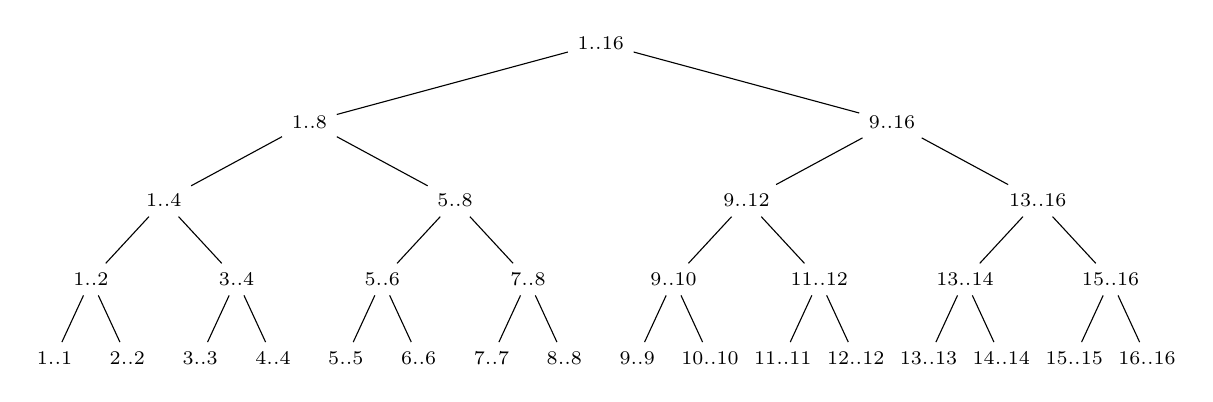
\begin{tikzpicture}[
	level/.append style = {level distance=10mm, sibling distance=148mm/2^#1},
	every node/.append style = {font=\scriptsize}
]

\node (root) {$1..16$}
	child {node {$1..8$}
		child {node {$1..4$}
			child {node {$1..2$}
				child {node {$1..1$}}
				child {node {$2..2$}}
			}
			child {node {$3..4$}
				child {node {$3..3$}}
				child {node {$4..4$}}
			}
		}
		child {node {$5..8$}
			child {node {$5..6$}
				child {node {$5..5$}}
				child {node {$6..6$}}
			}
			child {node {$7..8$}
				child {node {$7..7$}}
				child {node {$8..8$}}
			}
		}
	}
	child {node {$9..16$}
		child {node {$9..12$}
			child {node {$9..10$}
				child {node {$9..9$}}
				child {node {$10..10$}}
			}
			child {node {$11..12$}
				child {node {$11..11$}}
				child {node {$12..12$}}
			}
		}
		child {node {$13..16$}
			child {node {$13..14$}
				child {node {$13..13$}}
				child {node {$14..14$}}
			}
			child {node {$15..16$}
				child {node {$15..15$}}
				child {node {$16..16$}}
			}
		}
	};

\end{tikzpicture}

	\caption{Drzewo rekursji dla procedury \proc{Merge-Sort} działającej na tablicy z~16 elementami.
Każdy węzeł drzewa jest oznaczony przez zakres $i\twodots j$ tablicy, na której działa procedura.} \label{fig:15.3-2}
\end{figure}

\exercise %15.3-3
Problem ten ma własność optymalnej podstruktury, o~czym można się przekonać podobnie, jak w~jego oryginalnej wersji.
W~tym wariancie optymalnym nawiasowaniem iloczynu macierzy będziemy nazywać takie nawiasowanie, które maksymalizuje liczbę mnożeń skalarnych.

Przypuśćmy, że w~optymalnym nawiasowaniu iloczynu $A_iA_{i+1}\dots A_j$ podział występuje między $A_k$ i~$A_{k+1}$.
Wówczas nawiasowanie początkowego podciągu $A_iA_{i+1}\dots A_k$, stanowiące część optymalnego nawiasowania iloczynu $A_iA_{i+1}\dots A_j$, musi być optymalne.
Gdyby bowiem istniał sposób ustawienia nawiasów w~ciągu $A_iA_{i+1}\dots A_k$ o~większym koszcie, to podmieniając nawiasowanie tego podciągu w~optymalnym nawiasowaniu $A_iA_{i+1}\dots A_j$, otrzymalibyśmy inne nawiasowanie dla $A_iA_{i+1}\dots A_j$, ale o~koszcie większym niż optymalny, co stanowi sprzeczność z~założeniem.
Podobne rozumowanie prowadzi do wniosku, że nawiasowanie podciągu $A_{k+1}A_{k+2}\dots A_j$ w~optymalnym nawiasowaniu $A_iA_{i+1}\dots A_j$ jest optymalne dla ciągu $A_{k+1}A_{k+2}\dots A_j$.

\exercise %15.3-4
W~problemie planowania czynności na liniach montażowych zarówno najszybszy sposób montażu do stanowiska $S_{1,j}$, jak i~najszybszy sposób montażu do stanowiska $S_{2,j}$, polega na optymalnych czasach montażu do stanowisk $S_{1,j-1}$ i~$S_{2,j-1}$.
Innymi słowy, wartości $f_1[j-1]$ oraz $f_2[j-1]$ wykorzystywane są do obliczenia zarówno $f_1[j]$, jak i~$f_2[j]$.

\exercise %15.3-5
Jednym z~kontrprzykładów jest ciąg macierzy $\langle A_1,A_2,A_3\rangle$ o~rozmiarach stanowiących ciąg $\langle1,2,5,4\rangle$.
Liczbą mnożeń skalarnych wykonywanych podczas mnożenia $A_1$ przez $(A_2A_3)$ jest $1\cdot2\cdot4=8$, a~podczas mnożenia $(A_1A_2)$ przez $A_3$ -- $1\cdot5\cdot4=20$.
W~podejściu zachłannym podział iloczynu $A_1A_2A_3$ zostanie zatem wyznaczony między macierzą $A_1$ a~$A_2$ i~wynikowym nawiasowaniem będzie $(A_1(A_2A_3))$ z~kosztem $2\cdot5\cdot4+1\cdot2\cdot4=48$ mnożeń skalarnych.
Rozwiązaniem optymalnym jest jednak nawiasowanie $((A_1A_2)A_3)$ o~koszcie $1\cdot2\cdot5+1\cdot5\cdot4=30$.

\subchapter{Najdłuższy wspólny podciąg}

\exercise %15.4-1
Dla zadanych ciągów NWP wyznaczonym przez procedury \proc{LCS-Length} i~\proc{Print-LCS} jest $\langle1,0,0,1,1,0\rangle$.
Poza nim istnieje jeszcze 7 innych NWP tych ciągów:
\begin{gather*}
	\langle0,0,1,0,1,0\rangle, \langle0,0,1,0,1,1\rangle, \langle0,0,1,1,0,1\rangle, \langle0,1,0,1,0,1\rangle, \\
	\langle1,0,1,0,1,0\rangle, \langle1,0,1,0,1,1\rangle, \langle1,0,1,1,0,1\rangle.
\end{gather*}

\exercise %15.4-2
Poniższy pseudokod stanowi implementację zmodyfikowanej wersji procedury \proc{Print-LCS}, która wypisuje NWP ciągów $X$ i~$Y$ bez korzystania z~tablicy $b$.
Zamiast tego przyjmuje tablicę $c$ oraz dodatkowo ciąg $Y$.
Pierwsze wywołanie procedury powinno być następujące: $\proc{Print-LCS}'(c,X,Y,\attrib{X}{length},\attrib{Y}{length})$.
\begin{codebox}
\Procname{$\proc{Print-LCS}'(c,X,Y,i,j)$}
\li	\If $i=0$ lub $j=0$
\li		\Then \Return
		\End
\li	\If $x_i=y_j$
\li		\Then $\proc{Print-LCS}'(c,X,Y,i-1,j-1)$
\li			wypisz $x_i$
\li		\ElseIf $c[i,j]=c[i-1,j]$
\li			\Then $\proc{Print-LCS}'(c,X,Y,i-1,j)$
\li		\ElseNoIf $\proc{Print-LCS}'(c,X,Y,i,j-1)$
		\End
\end{codebox}

\exercise %15.4-3
W~naszej implementacji będziemy obliczać kolejne wartości rekurencyjnie bezpośrednio ze wzoru (15.14), ale z~wykorzystaniem tablicy $c[0\twodots m,0\twodots n]$ i~mechanizmu spamiętywania.
Aby zaznaczyć, że dane pole tablicy $c$ nie zostało jeszcze obliczone, użyjemy specjalnej wartości $\infty$.
Pierwsza z~procedur inicjalizuje tablicę $c$, po czym wywołuje właściwy algorytm odpowiedzialny za obliczenie wartości $c[m,n]$.
\begin{codebox}
\Procname{$\proc{Memoized-LCS-Length}(X,Y)$}
\li	$m\gets\attrib{X}{length}$
\li	$n\gets\attrib{Y}{length}$
\li	\For $i\gets0$ \To $m$
\li		\Do \For $j\gets0$ \To $n$
\li				\Do $c[i,j]\gets\infty$ \label{li:memoized-lcs-length-init}
				\End
		\End
\li	\Return $\proc{Lookup-LCS}(c,X,Y,m,n)$
\end{codebox}
\begin{codebox}
\Procname{$\proc{Lookup-LCS}(c,X,Y,i,j)$}
\li	\If $c[i,j]<\infty$
\li		\Then \Return $c[i,j]$
		\End
\li	\If $i=0$ lub $j=0$
\li		\Then $c[i,j]\gets0$
\li		\ElseIf $x_i=y_j$
\li			\Then $c[i,j]\gets\proc{Lookup-LCS}(c,X,Y,i-1,j-1)+1$
\li		\ElseNoIf $c[i,j]\gets\max(\proc{Lookup-LCS}(c,X,Y,i,j-1),\proc{Lookup-LCS}(c,X,Y,i-1,j))$
		\End
\li	\Return $c[i,j]$
\end{codebox}

Każde z~$(m+1)(n+1)$ pól tablicy $c$ zostaje zainicjalizowane w~wierszu \ref{li:memoized-lcs-length-init} pierwszej procedury, a~następnie zmodyfikowane przez jedno wywołanie algorytmu \proc{Lookup-LCS}.
Wywołania \proc{Lookup-LCS} możemy podzielić na dwa typy:
\begin{enumerate}
	\renewcommand{\labelenumi}{(\roman{enumi})}
	\item wywołania, w~których $c[i,j]=\infty$, oraz
	\item wywołania, w~których $c[i,j]<\infty$.
\end{enumerate}
Wywołań pierwszego typu jest dokładnie $\Theta(mn)$, jedno na każde pole tablicy $c$, a~każde z~nich jest wykonywane w~czasie $\Theta(1)$ plus czas spędzany na obliczenia rekurencyjne.
Do każdego wywołania drugiego typu może doprowadzić rekursja podczas wywołania pierwszego typu.
Kiedy w~danym wywołaniu \proc{Lookup-LCS} pojawiają się wywołania rekurencyjne, jest ich $\Theta(1)$, dlatego łącznie wywołań drugiego typu jest $\Theta(mn)$, z~których każde zabiera czas $\Theta(1)$.
Stąd całkowity czas wykonania procedury \proc{Memoized-LCS-Length} wynosi $\Theta(mn)$.

\exercise %15.4-4
Zauważmy, że do obliczenia $c[i,j]$ w~procedurze \proc{LCS-Length} wykorzystywane są wartości $c[i-1,j]$, $c[i,j-1]$ oraz $c[i-1,j-1]$.
Możemy więc utrzymywać tylko 2 wiersze tablicy $c$ -- wiersz aktualnie obliczany oraz wiersz bezpośrednio go poprzedzający.
Po każdej iteracji poprzedni wiersz będzie nadpisywany wartościami z~bieżącego wiersza, aby przygotować tablicę do kolejnej iteracji.
Aby tablica $c$ była rozmiaru $2\cdot\min(m,n)$, przed jej utworzeniem należy jeszcze sprawdzić, czy $n\le m$.
Jeśli nie, to wystarczy uruchomić procedurę z~ciągami $X$ i~$Y$ zamienionymi miejscami.

Można jednak jeszcze bardziej ograniczyć zapotrzebowanie procedury na pamięć.
Dwuwymiarowa tablica $c$ może zostać zamieniona na jednowymiarową tablicę $C[1\twodots n]$, która reprezentować będzie aktualnie obliczany wiersz tablicy $c$ w~trakcie działania procedury.
W~momencie obliczania $c[i,j]$ reprezentowanego przez $C[j]$, komórka $C[j]$ przechowuje wartość $c[i-1,j]$ z~poprzedniego wiersza.
Jeśli w~osobnej zmiennej $p$ zapamiętamy $c[i-1,j-1]$, czyli wartość $C[j-1]$ przed jej aktualizacją, to będziemy dysponować wszystkimi danymi potrzebnymi do obliczenia $C[j]$.
Jeśli $x_i=y_j$, to $C[j]$ ustawione zostanie na $p+1$, co odpowiada wierszowi 10 z~oryginalnej procedury \proc{LCS-Length}.
W~przeciwnym przypadku do $C[j]$ wpisane zostanie $\max(C[j],C[j-1])$, co odpowiada wierszom \doubledash{12}{16}.
Ostatnim krokiem w~bieżącej iteracji pętli jest aktualizacja zmiennej $p$ na wartość znajdującą się w~$C[j]$ przed modyfikacją tej komórki.
Dzięki tak wprowadzonym zmianom w~procedurze wykorzystujemy $\min(m,n)+\Theta(1)$ pamięci.

\exercise %15.4-5
W~\textbf{problemie najdłuższego niemalejącego podciągu} (w~skrócie: problemu NNP) dla danego ciągu $X=\langle x_1,x_2,\dots,x_n\rangle$ szukany jest podciąg ciągu $X$ o~największej możliwej długości, którego wyrazy ustawione są w~porządku niemalejącym.
Przez $c[i]$ oznaczmy długość najdłuższego niemalejącego podciągu ciągu $X$, w~którym ostatnim wyrazem jest $x_i$.
NNP ciągu $X$ zakończony wyrazem $x_i$ składa się z~NNP prefiksu $X_{i-1}$ z~dołączonym na końcu $x_i$, o~ile tylko NNP prefiksu $X_{i-1}$ zakończony jest wyrazem $x_j\le x_i$.
Jeśli nie istnieje takie $1\le j<i$, to NNP ciągu $X$ jest $\langle x_i\rangle$.
Problem ma zatem własność optymalnej podstruktury.
Aby znaleźć długość NNP danego ciągu, należy wpierw znaleźć rozwiązania podproblemów, czyli długości NNP prefiksów tego ciągu.
Otrzymujemy zależność rekurencyjną:
\[
	c[i] = \begin{cases}
		1, & \text{jeśli $x_j>x_i$ dla każdego $1\le j<i$}, \\
		\displaystyle\max_{\substack{1\le j<i\\x_j\le x_i}}(c[j])+1, & \text{w~przeciwnym przypadku}.
	\end{cases}
\]
NNP ciągu $X$ ma wówczas długość $\max_{1\le i\le n}c[i]$.

Obliczanie wartości tablicy $c$ bezpośrednio z~definicji doprowadziłoby do algorytmu o~czasie wykładniczym z~racji wielokrotnego rozwiązywania tych samych podproblemów.
Dzięki wykorzystaniu tablicowania wyników w~programowaniu dynamicznym, możemy podać algorytm działający w~czasie $O(n^2)$.
\begin{codebox}
\Procname{$\proc{LIS-Length}(X)$}
\li	$n\gets\attrib{X}{length}$
\li	$m\gets0$
\li	$b^*\!\gets0$
\li	\For $i\gets1$ \To $n$ \label{li:lis-length-computing-c-begin}
\li		\Do $c[i]\gets1$
\li			$b[i]\gets0$
\li			\For $j\gets1$ \To $i-1$
\li				\Do \If $x_j\le x_i$ i~$c[j]+1>c[i]$
\li						\Then $c[i]\gets c[j]+1$
\li							$b[i]\gets j$
						\End
				\End
\li			\If $c[i]>m$
\li				\Then $m\gets c[i]$
\li					$b^*\!\gets i$
				\End
		\End \label{li:lis-length-computing-c-end}
\li	\Return $m$, $b$ i~$b^*$
\end{codebox}
W~pętli \kw{for} w~wierszach \doubledash{\ref{li:lis-length-computing-c-begin}}{\ref{li:lis-length-computing-c-end}} wyznaczane są kolejne pola tablicy $c$, a~także aktualizowana jest zmienna $m$ przechowująca długość najdłuższego aktualnie znanego niemalejącego podciągu wejściowego ciągu $X$.
W~tablicy $b[1\twodots n]$ zapamiętywane są dodatkowe informacje służące później do odtworzenia znalezionego NNP.
Dokładniej, po zakończeniu działania procedury, na pozycji $b[i]$ znajduje się taka wartość $j$, dla której $c[i]=c[j]+1$, albo $b[i]=0$, jeżeli takie $j$ nie istnieje.
Ponadto, $b^*\!$ przechowuje takie $i$, dla którego $m=c[i]$, albo 0, jeżeli ciąg $X$ jest pusty.

Znaleziony podciąg można otrzymać (w~odwrotnej kolejności) poprzez wypisanie $x_{b^*\!}$, a~następnie $x_{b[b^*\!]}$, $x_{b[b[b^*\!]]}$ itd., dopóki indeks nie jest zerem.
Następująca rekurencyjna procedura pozwala wypisać NNP we właściwej kolejności.
\begin{codebox}
\Procname{$\proc{Print-LIS}(b,X,i)$}
\li	\If $b[i]>0$
\li		\Then $\proc{Print-LIS}(b,X,b[i])$
		\End
\li	wypisz $x_i$
\end{codebox}
Dysponując tablicą $b$ i~wartością $b^*\!$ wyznaczonymi dla danego ciągu $X$, możemy wypisać jego NNP, wywołując $\proc{Print-LIS}(b,X,b^*\!)$.

\exercise %15.4-6
Dla ciągu wejściowego $X=\langle x_1,x_2,\dots,x_n\rangle$, w~którym NNP ma długość $m$, niech $Z=\langle z_1,z_2,\dots,z_m\rangle$ będzie ciągiem takim, że $z_i$ jest najmniejszym elementem w~$X$ kończącym pewien podciąg niemalejący ciągu $X$ o~długości $i$.
Kluczowa jest własność ciągu $Z$ podana we wskazówce, czyli to, że jest on niemalejący.
Podamy krótki dowód tego faktu.
Załóżmy nie-wprost, że istnieją indeksy $i$, $j$, takie, że $i<j$ oraz $z_i>z_j$.
Oznacza to, że najmniejszy element ciągu $X$ będący ostatnim elementem niemalejącego podciągu $X$ o~długości $i$ jest większy niż najmniejszy element ciągu $X$ kończący pewien niemalejący podciąg $X$ o~długości $j$.
Moglibyśmy jednak usunąć $j-i$ elementów z~podciągu o~długości $j$ zakończonego na $z_j$, otrzymując niemalejący podciąg ciągu $X$ o~długości $i$, w~którym ostatni element jest mniejszy niż $z_i$.
Sprzeczność.

Zamiast zapamiętywania ciągu $Z$, w~algorytmie będziemy korzystać z~tablicy $a[0\twodots n]$, w~której na \singledash{$j$}{tej} pozycji, gdzie $j=1$, 2, \dots, $m$, będziemy przechowywać indeks $i$, taki że $z_j=x_i$.
Dla pozycji $j=0$ oraz $j=m+1$, $m+2$, \dots, $n$, przyjmiemy $a[j]=0$.
Przechowywanie indeksów elementów pozwoli nam na zbudowanie tablicy $b$ identycznej, jak w~procedurze \proc{LIS-Length} z~poprzedniego zadania, dzięki której będzie można odtworzyć znaleziony NNP.

Załóżmy, że w~trakcie przeglądania ciągu $X$ od lewej do prawej, aktualnie przetwarzanym elementem jest $x_i$, a~w~zmiennej $m$ przechowywana jest długość najdłuższego aktualnie znanego niemalejącego podciągu $X$.
Niech $k$ będzie takim indeksem w~tablicy $a$, że $x_{a[j]}\le x_i$ dla każdego $j=1$, 2, \dots, $k-1$, oraz $x_{a[j]}>x_i$ dla każdego $j=k$, $k+1$, \dots, $m$.
Element $x_i$ stanowi zatem najmniejszy napotkany do tej pory element kończący pewien niemalejący podciąg ciągu $X$ o~długości $k$ -- na pozycję $a[k]$ można więc wpisać $i$.
Dzięki uporządkowaniu elementów ciągu $X$ o~indeksach z~tablicy $a$, liczbę $k$ dla każdego elementu $x_i$ jesteśmy w~stanie wyznaczać w~czasie logarytmicznym, stosując wyszukiwanie binarne.

\begin{codebox}
\Procname{$\proc{LIS-Length}'(X)$}
\li	$n\gets\attrib{X}{length}$
\li	\For $i\gets0$ \To $n$ \label{li:lis-length'-a-init-begin}
\li		\Do $a[i]\gets0$
		\End \label{li:lis-length'-a-init-end}
\li	$m\gets0$
\li	\For $i\gets1$ \To $n$ \label{li:lis-length'-for-begin}
\li		\Do $k\gets1$ \label{li:lis-length'-binary-search-begin}
\li			$l\gets m$
\li			\While $k\le l$
\li				\Do $j\gets\lfloor(k+l)/2\rfloor$
\li					\If $x_{a[j]}\le x_i$
\li						\Then $k\gets j+1$
\li						\Else $l\gets j-1$
						\End
				\End \label{li:lis-length'-binary-search-end}
\li			$a[k]\gets i$
\li			$b[i]\gets a[k-1]$
\li			\If $k>m$
\li				\Then $m\gets k$
				\End
		\End \label{li:lis-length'-for-end}
\li	\Return $m$, $b$ i~$a[m]$
\end{codebox}
Powyżej zaprezentowany algorytm realizuje opisane podejście.
W~wierszach \doubledash{\ref{li:lis-length'-a-init-begin}}{\ref{li:lis-length'-a-init-end}} tablica $a$ inicjalizowana jest zerami, aby zaznaczyć, że żaden z~elementów ciągu $Z$ nie jest jeszcze znany.
Elementy ciągu $X$ przeglądane są następnie od lewej do prawej.
W~wierszach \doubledash{\ref{li:lis-length'-binary-search-begin}}{\ref{li:lis-length'-binary-search-end}} dla elementu $x_i$ odbywa się wyszukiwanie odpowiedniego indeksu tablicy $a$, gdzie należy umieścić $i$, aby zachować uporządkowanie elementów ciągu $X$ indukowane przez fragment $a[1\twodots m]$.
Po aktualizacji odpowiedniej komórki tablicy $a$, do $b[i]$ wpisywany jest indeks poprzedniego elementu w~ciągu $Z$ (lub 0, jeśli element $x_i$ rozpoczyna nowy podciąg niemalejący), a~następnie aktualizowana jest wartość zmiennej $m$.
Procedura zwraca ten sam zestaw wyników, co \proc{LIS-Length} z~poprzedniego zadania (z~$a[m]$ jako $b^*\!$).
Znaleziony NNP można więc wypisać, wywołując procedurę \proc{Print-LIS} tak, jak to opisano w~tamtym rozwiązaniu.

Każda iteracja pętli \kw{for} w~liniach \doubledash{\ref{li:lis-length'-for-begin}}{\ref{li:lis-length'-for-end}} przeprowadza wyszukiwanie binarne w~podtablicy zawierającej co najwyżej $n$ elementów.
Poza pętlą inicjalizującą tablicę $a$ pozostałe operacje wykonywane w~procedurze zajmują czas co najwyżej stały.
Stąd algorytm działa w~czasie $O(n\lg n)$.

\subchapter{Optymalne drzewa wyszukiwań binarnych}

\exercise %15.5-1
Algorytm podzielimy na 3 procedury.
Pierwsza z~nich ma za zadanie wypisać korzeń optymalnego drzewa BST oraz wywołać drugą, rekurencyjną procedurę wypisującą strukturę tego drzewa.
W~tym celu dla danej tablicy \id{root} oraz pozycji $i\le j$ konstruowane jest poddrzewo o~korzeniu, którego indeks znajduje się w~$\id{root}[i,j]$.
Konstrukcja ta polega na wypisaniu jego lewego poddrzewa, a~następnie na wypisaniu jego prawego poddrzewa.
Trzecia procedura służy nam do pozyskiwania nazw węzłów na podstawie wartości w~tablicy \id{root} oraz pozycji w~niej.
\begin{codebox}
\Procname{$\proc{Construct-Optimal-BST}(\id{root})$}
\li	$n\gets\attribii{root}{length}$
\li	wypisz $\proc{Optimal-BST-Node}(\id{root},i,n)$ ,, jest korzeniem''
\li	$\proc{Construct-Optimal-BST-Subtree}(\id{root},1,n)$
\end{codebox}
\begin{codebox}
\Procname{$\proc{Construct-Optimal-BST-Subtree}(\id{root},i,j)$}
\li	\If $i\le j$
\li		\Then wypisz $\proc{Optimal-BST-Node}(\id{root},i,\id{root}[i,j]-1)$ ,, jest lewym synem $k$''$\!{}_{\id{root}[i,j]}$
\li			$\proc{Construct-Optimal-BST-Subtree}(\id{root},i,\id{root}[i,j]-1)$
\li			wypisz $\proc{Optimal-BST-Node}(\id{root},\id{root}[i,j]+1,j)$ ,, jest prawym synem $k$''$\!{}_{\id{root}[i,j]}$
\li			$\proc{Construct-Optimal-BST-Subtree}(\id{root},\id{root}[i,j]+1,j)$
		\End
\end{codebox}
\begin{codebox}
\Procname{$\proc{Optimal-BST-Node}(\id{root},i,j)$}
\li	\If $i\le j$
\li		\Then \Return ,,$k$''$\!{}_{\id{root}[i,j]}$
\li		\Else \Return ,,$d$''$\!{}_j$
		\End
\end{codebox}

\exercise %15.5-2
Algorytm \proc{Optimal-BST} wywołany dla zadanych prawdopodobieństw zwraca optymalne drzewo BST przedstawione na rys.\ \ref{fig:15.5-2}.
Tabela \ref{tab:15.5-2} ilustruje, podobnie jak w~Podręczniku, oczekiwany koszt wyszukiwania w~tym drzewie oraz wkład, jaki wprowadza w~ten koszt każdy węzeł.
\begin{figure}[!ht]
	\centering \begin{tikzpicture}[
	level/.append style = {level distance=7mm, sibling distance=120mm/2^#1},
	every node/.style = {tree node}
]

\newcommand\leafnode[1]{%
	node[align=center, inner sep=1pt, minimum size=5mm, rectangle, rounded corners=3pt, draw] {#1}
}

\node (root) {$k_5$}
	child {node {$k_2$}
		child {node {$k_1$}
			child[shorten >=-1pt] {\leafnode {$d_0$}}
			child[shorten >=-1pt] {\leafnode {$d_1$}}
		}
		child {node {$k_3$}
			child[shorten >=-1pt] {\leafnode {$d_2$}}
			child {node {$k_4$}
				child {\leafnode {$d_3$}}
				child {\leafnode {$d_4$}}
			}
		}
	}
	child {node {$k_7$}
		child {node {$k_6$}
			child[shorten >=-1pt] {\leafnode {$d_5$}}
			child [shorten >=-1pt]{\leafnode {$d_6$}}
		}
		child {\leafnode {$d_7$}}
	};

\end{tikzpicture}

	\caption{Optymalne drzewo BST dla zadanego ciągu prawdopodobieństw.} \label{fig:15.5-2}
\end{figure}
\begin{table}[!ht]
	\centering
		\begin{tabular}{cccc}
			węzeł & głębokość & prawdopodobieństwo & wkład \\ \hline
			$k_1$ & 2 & 0{,}04 & 0{,}12 \\
			$k_2$ & 1 & 0{,}06 & 0{,}12 \\
			$k_3$ & 2 & 0{,}08 & 0{,}24 \\
			$k_4$ & 3 & 0{,}02 & 0{,}08 \\
			$k_5$ & 0 & 0{,}10 & 0{,}10 \\
			$k_6$ & 2 & 0{,}12 & 0{,}36 \\
			$k_7$ & 1 & 0{,}14 & 0{,}28 \\
			$d_0$ & 3 & 0{,}06 & 0{,}24 \\
			$d_1$ & 3 & 0{,}06 & 0{,}24 \\
			$d_2$ & 3 & 0{,}06 & 0{,}24 \\
			$d_3$ & 4 & 0{,}06 & 0{,}30 \\
			$d_4$ & 4 & 0{,}05 & 0{,}25 \\
			$d_5$ & 3 & 0{,}05 & 0{,}20 \\
			$d_6$ & 3 & 0{,}05 & 0{,}20 \\
			$d_7$ & 2 & 0{,}05 & 0{,}15 \\ \hline
			Razem & & & 3{,}12
		\end{tabular} \caption{Zestawienie kosztów wprowadzanych przez poszczególne węzły w~optymalnym drzewie BST dla podanych prawdopodobieństw.} \label{tab:15.5-2}
\end{table}

\exercise %15.5-3
Obliczanie wartości $w(i,j)$ bezpośrednio ze wzoru (15.17) wymaga wykonania $\Theta(j-i)$ dodawań.
Zauważmy, że pętla \kw{for} w~wierszach \doubledash{9}{13} wykonuje także $\Theta(j-i)$ iteracji, a~każda z~nich wymaga czasu stałego.
A~zatem modyfikacja ta nie wpłynie na asymptotyczny czas działania algorytmu, tylko co najwyżej na zwiększenie stałego czynnika ukrytego w~notacji $\Theta$.

\exercise %15.5-4
Wykorzystamy podaną obserwację i~w~najbardziej wewnętrznej pętli w~procedurze \proc{Optimal-BST}, zamiast iterować zmienną $r$ od $i$ do $j$, będziemy przebiegać wszystkie wartości od $\id{root}[i,j-1]$ do $\id{root}[i+1,j]$.
Aby jednak skorzystać z~tego usprawnienia, musimy upewnić się, że $i<j$.
Warunek ten zachodzi, gdy $l>1$, zatem w~pętli \kw{for} w~wierszach \doubledash{4}{13} zmienna $l$ będzie przyjmować wartości od 2 do $n$, natomiast działania wykonywane, gdy $l=1$, będziemy imitować następującym fragmentem, który wstawimy tuż przed tę pętlę:
\begin{codebox}
\zi	\For $i\gets1$ \To $n$
\zi		\Do $w[i,i]\gets w[i,i-1]+p_i+q_i$
\zi			$e[i,i]\gets e[i,i-1]+e[i+1,i]+w[i,i]$
\zi			$\id{root}[i,i]\gets i$
		\End
\end{codebox}

Pokażemy, że tablice $e$ i~\id{root} zostaną wypełnione w~czasie $\Theta(n^2)$.
Pętla w~wierszach \doubledash{1}{3} wraz z~tą stanowiącą nowy fragment wykonują w~sumie $2n+1$ iteracji.
Dla każdego $2\le l\le n$ pętla \kw{for} w~wierszach \doubledash{9}{13} wykona łącznie $S(n,l)=\sum_{i=1}^{n-l+1}(\id{root}[i+1,j]-\id{root}[i,j-1]+1)$ iteracji.
Po podstawieniu $j=i+l-1$ i~skorzystaniu z~własności sumy teleskopowej otrzymujemy:
\begin{align*}
	S(n,l) &= \sum_{i=1}^{n-l+1}(\id{root}[i+1,j]-\id{root}[i,j-1]+1) \\
	&= \sum_{i=1}^{n-l+1}(\id{root}[i+1,i+l-1]-\id{root}[i,i+l-2])+\sum_{i=1}^{n-l+1}1 \\
	&= \id{root}[n-l+2,n]-\id{root}[1,l-1]+n-l+1.
\end{align*}
Największą możliwą wartością różnicy $\id{root}[n-l+2,n]-\id{root}[1,l-1]$ jest $n-1$, skąd mamy $S(n,l)\le n-1+n-l+1\le2n-2$.
Sumaryczna liczba iteracji najbardziej wewnętrznej pętli wynosi więc $\sum_{l=2}^nS(n,l)\le2(n-1)^2=O(n^2)$.
Obliczana jest każda z~$n(n+1)/2$ z~komórek tablic $e$ i~\id{root}, dlatego dolnym ograniczeniem na czas potrzebny do ich wypełnienia jest oczywiście $\Omega(n^2)$.
Stąd czasem działania algorytmu jest $\Theta(n^2)$.


\problems

\problem{Bitoniczny problem komiwojażera} %15-1
W~naszym rozwiązaniu przyjmujemy, że żadne dwa punkty wejściowe nie mają tej samej współrzędnej $x$.
Podążając za wskazówką z~treści problemu, będziemy przeglądać punkty wejściowe od lewej do prawej, po uprzednim posortowaniu ich po współrzędnych $x$.
Ciąg tak uporządkowanych punktów oznaczymy przez $\langle p_1,p_2,\dots,p_n\rangle$, czyli $p_1$ jest punktem wysuniętym najbardziej na lewo, a~$p_n$ punktem wysuniętym najbardziej na prawo.

Oznaczmy przez $B_{i,j}$, gdzie $i\le j$, zbiór ścieżek bitonicznych zawierających wszystkie punkty $p_1$, $p_2$, \dots, $p_j$, które zaczynają się w~pewnym punkcie $p_i$, biegną następnie ciągle w~lewo (czyli po punktach o~coraz mniejszych współrzędnych $x$) do punktu $p_1$, a~następnie ciągle w~prawo (czyli po punktach o~coraz większych współrzędnych $x$) do punktu $p_j$.
Przez $|p_ip_j|$ oznaczymy odległość euklidesową między punktami $p_i$ i~$p_j$, a~przez $b[i,j]$, gdzie $1\le i\le j\le n$, długość najkrótszej ścieżki bitonicznej ze zbioru $B_{i,j}$.
Zauważmy, że zbiór $B_{1,j}$ zawiera tylko jedną ścieżkę, dlatego $b[1,j]=\sum_{k=2}^j|p_{k-1}p_k|$.
Jedyną wartością $b[i,i]$, której będziemy potrzebować, jest $b[n,n]$, co stanowi długość szukanego najkrótszego cyklu bitonicznego dla wejściowego zbioru punktów.

Rozważmy najkrótszą ścieżkę bitoniczną $\beta$ z~$B_{i,j}$ i~zastanówmy się nad położeniem na niej punktu $p_{j-1}$.
Jeśli znajduje się on na podścieżce biegnącej w~prawo, to poprzedza on bezpośrednio punkt $p_j$ na tej podścieżce.
Podścieżka od $p_i$ do $p_{j-1}$ musi być najkrótszą ścieżką bitoniczną z~$B_{i,j-1}$, inaczej moglibyśmy ją ,,wyciąć'' i~,,wkleić'' w~jej miejsce podścieżkę bitoniczną o~mniejszej długości, uzyskując ścieżkę krótszą niż $\beta$.
Stąd długość $b[i,j]$ ścieżki $\beta$ wynosi $b[i,j-1]+|p_{j-1}p_j|$.
W~przeciwnym przypadku $p_{j-1}$ musi być najbardziej w~prawo wysuniętym punktem podścieżki biegnącej w~lewo, czyli $i=j-1$.
Bezpośrednio przed $p_j$ na podścieżce biegnącej w~prawo mamy więc $p_k$, gdzie $k<j-1$.
Tutaj także ma miejsce optymalna podstruktura -- podścieżka z~$p_k$ do $p_{j-1}$ jest najkrótszą ścieżką bitoniczną z~$B_{k,j-1}$, o~czym można się przekonać stosując metodę ,,wytnij i~wklej''.
W~tym przypadku ścieżka $\beta$ ma długość $b[i,j]=\min_{1\le k<j-1}(b[k,j-1]+|p_kp_j|)$.
Zachodzi zatem następująca zależność rekurencyjna:
\[
	b[i,j] = \begin{cases}
		|p_1p_2|, & \text{jeśli $i=1$, $j=2$}, \\
		\displaystyle\min_{1\le k<j-1}(b[k,j-1]+|p_kp_j|), & \text{jeśli $i=j-1>1$}, \\
		b[i,j-1]+|p_{j-1}p_j|, & \text{jeśli $i<j-1$}.
	\end{cases}
\]
W~szukanym optymalnym cyklu bitonicznym, jednym z~punktów sąsiadujących z~$p_n$ jest $p_{n-1}$, skąd $b[n,n]=b[n,n-1]+|p_{n-1}p_n|$.

Aby zrekonstruować rozwiązanie, będziemy obliczać wartości $r[i,j]$ -- indeks punktu bezpośrednio poprzedzającego $p_j$ na najkrótszej ścieżce z~$B_{i,j}$.
Poniższy pseudokod wyznacza wartości $b[i,j]$ i~$r[i,j]$, wykorzystując programowanie dynamiczne.
\begin{codebox}
\Procname{$\proc{Bitonic-TSP}(p,n)$}
\li	posortuj ciąg punktów wejściowych $p$ rosnąco względem ich współrzędnych $x$
\li	$b[1,2]\gets|p_1p_2|$
\li	\For $j\gets3$ \To $n$
\li		\Do \For $i\gets1$ \To $j-2$
\li			\Do $b[i,j]\gets b[i,j-1]+|p_{j-1}p_j|$
\li				$r[i,j]\gets j-1$
			\End
\li			$b[j-1,j]\gets\infty$
\li			\For $k\gets1$ \To $j-2$
\li				\Do $q\gets b[k,j-1]+|p_kp_j|$
\li					\If $q<b[j-1,j]$
\li						\Then $b[j-1,j]\gets q$
\li							$r[j-1,j]\gets k$
						\End
				\End
		\End
\li	$b[n,n]\gets b[n,n-1]+|p_{n-1}p_n|$
\li	\Return $b$ i~$r$
\end{codebox}

Znalezione rozwiązanie wypiszemy, zaczynając od $p_n$, następnie wypiszemy punkty na podścieżce biegnącej w~lewo, która zawiera $p_{n-1}$, aż do $p_1$, a~następnie pozostałe punkty z~podścieżki biegnącej w~prawo aż do $p_n$.
\begin{codebox}
\Procname{$\proc{Print-Bitonic-Tour}(r,n)$}
\li	wypisz $p_n$
\li	wypisz $p_{n-1}$
\li	$\proc{Print-Bitonic-Path}(r,r[n-1,n],n-1)$
\li	wypisz $p_{r[n-1,n]}$
\end{codebox}
\begin{codebox}
\Procname{$\proc{Print-Bitonic-Path}(r,i,j)$}
\li	\If $i<j$
\li		\Then wypisz $p_{r[i,j]}$
\li			\If $r[i,j]>1$
\li				\Then $\proc{Print-Bitonic-Path}(r,i,r[i,j])$
				\End
\li		\Else \If $r[j,i]>1$
\li				\Then $\proc{Print-Bitonic-Path}(r,r[j,i],j)$
\li					wypisz $p_{r[j,i]}$
				\End
		\End
\end{codebox}
W~wywołaniu $\proc{Print-Bitonic-Path}(r,i,j)$, jeśli $i<j$, to procedura ta wypisuje podścieżkę biegnącą w~lewo, a~jeśli $i>j$, to podścieżkę biegnącą w~prawo.

Czas działania algorytmu \proc{Bitonic-TSP} wynosi $O(n^2)$, gdyż zewnętrzna pętla wykonuje $n-2$ iteracje, a~każda wewnętrzna pętla wykonuje co najwyżej $n-2$ iteracji.
Sortowanie punktów na samym początku algorytmu można wykonać w~czasie $O(n\lg n)$, co nie wpływa na powyższe oszacowanie.
Wypisanie znalezionego cyklu za pomocą procedury \proc{Print-Tour} odbywa się w~czasie $O(n)$, dlatego że każdy punkt wypisywany jest dokładnie raz.

\problem{Estetyczny wydruk} %15-2
Danymi wejściowymi w~naszym rozwiązaniu będzie ciąg $l$ długości słów wejściowych oraz pojemność wiersza $M$.
Przedstawiony algorytm można nietrudno przekształcić tak, aby przyjmował rzeczywisty akapit tekstu i~wypisywał jego słowa podzielone na linie.
Zakładamy ponadto, że każde słowo z~tego akapitu mieści się w~wierszu, tzn.\ $l_i\le M$ dla każdego $i=1$, 2, \dots, $n$.

Zdefiniujmy $\id{extras}[i,j]$, gdzie $i\le j$, jako liczbę zbędnych znaków odstępu na końcu wiersza zawierającego słowa o~numerach od $i$ do $j$, czyli $\id{extras}[i,j]=M-j+i-\sum_{k=i}^jl_k$.
Z~kolei $\id{lc}[i,j]$ niech będzie kosztem wprowadzanym przez wiersz ze słowami od $i$ do $j$.
Przyjmiemy, że $\id{lc}[i,j]=\infty$, jeśli słowa te nie mieszczą się w~wierszu -- taki zabieg sprawi, że podczas minimalizacji tych wartości przepełnione wiersze nie będą wybierane.
Ostatni wiersz, jeśli nie jest przepełniony, wprowadza zerowy koszt, zgodnie ze specyfikacją problemu.
Mamy więc:
\[
	\id{lc}[i,j] = \begin{cases}
		\infty, & \text{jeśli $\id{extras}[i,j]<0$}, \\
		0, & \text{jeśli $j=n$ i~$\id{extras}[i,j]\ge0$}, \\
		(\id{extras[i,j]})^3, & \text{w~pozostałych przypadkach}.
	\end{cases}
\]

Naszym zadaniem jest minimalizacja sumy wartości \id{lc} po wszystkich wierszach, na jakie można podzielić tekst wejściowy.
Rozważmy optymalne rozmieszczenie słów o~numerach od 1 do $j$, gdzie $1\le j\le n$.
Niech $i$ będzie numerem słowa, które rozpoczyna ostatni wiersz w~takim podziale.
Poprzednie wiersze, o~ile istnieją, składają się zatem ze słów od 1 do $i-1$ i~rozmieszczenie ich w~wierszach musi być optymalne, co można uzasadnić za pomocą metody ,,wytnij i~wklej''.
Niech $c[j]$ będzie kosztem optymalnego układu słów od 1 do $j$.
Jeśli ostatni wiersz rozpoczyna słowo o~numerze $i$, to $c[j]=c[i-1]+\id{lc}[i,j]$.
Odpowiednią wartość $i$ minimalizującą $c[j]$ można wyznaczyć, sprawdzając każdy numer od 1 do $j$ i~wybierając optymalny z~nich.
Możemy ponadto przyjąć $c[0]=0$ jako brzegowy przypadek tej rekurencji:
\[
	c[j] = \begin{cases}
		0, & \text{jeśli $j=0$}, \\
		\displaystyle\min_{1\le i\le j}(c[i-1]+\id{lc}[i,j]), & \text{jeśli $j>0$}.
	\end{cases}
\]
Jej wartości możemy przechowywać w~tablicy i~obliczać od lewej do prawej.

Zaobserwujmy jednak, że wiersz może zawierać co najwyżej $\lceil M/2\rceil$ słów.
W~wierszu składającym się z~$j-i+1$ słów o~numerach od $i$ do $j$, jeśli $j-i+1>\lceil M/2\rceil$, to wiadomo, że $\id{lc}[i,j]=\infty$.
Stąd podczas obliczania $c[j]$ można tak naprawdę ograniczyć zakres sprawdzanych numerów $i$ od dołu przez $\max(1,j-\lceil M/2\rceil+1)$.

Zauważmy też, że możemy zrezygnować z~tablic \id{extras} oraz \id{lc} i~pamiętać jedynie potrzebne w~danej chwili wartości.
Posłużymy się w~tym celu ciągiem sum prefiksowych długości słów, który przechowamy w~tablicy $L[0\twodots n]$.
Dokładniej, dla każdego $j=0$, 1, \dots, $n$, $L[j]=\sum_{k=1}^jl_k$.
Zdefiniowane wcześniej $\id{extras}[i,j]$ wynosi wówczas $M-j+i-(L[j]-L[i-1])$ i~wartość tę można wyznaczyć w~czasie stałym.
Podobnie wartości z~tablicy \id{lc} można wyliczać na bieżąco, ponieważ w~danym momencie wykorzystywana jest tylko jedna z~nich.

Do zapamiętywania, na~których pozycjach wejściowego ciągu następuje podział na wiersze, wykorzystamy dodatkową tablicę $p$.
W~trakcie obliczania $c[j]$, jeśli $c[j]=c[i-1]+\id{lc}[i,j]$, to do $p[j]$ wpiszemy $i$.
Dzięki temu będziemy wiedzieć, że ostatni wiersz w~znalezionym rozwiązaniu zawiera słowa o~numerach od $p[n]$ do $n$, przedostatni -- słowa o~numerach od $p[p[n]-1]$ do $p[n]-1$ itd.

\begin{codebox}
\Procname{$\proc{Break-Lines}(l,M)$}
\li	$n\gets\attrib{l}{length}$
\li	$L[0]\gets0$
\li	\For $i\gets1$ \To $n$
\li		\Do $L[i]\gets L[i-1]+l_i$
		\End
\li	$c[0]\gets0$
\li	\For $j\gets1$ \To $n$
\li		\Do $c[j]\gets\infty$
\li			$j_0\gets\max(1,j-\lceil M/2\rceil+1)$
\li			\For $i\gets j_0$ \To $j$
\li				\Do $\id{extras}\gets M-j+i-(L[j]-L[i-1])$
\li					\If $\id{extras}<0$
\li						\Then $\id{lc}\gets\infty$
\li					\ElseIf $j=n$
\li						\Then $\id{lc}\gets0$
\li					\ElseNoIf $\id{lc}\gets\id{extras}^3$
						\End
\li					\If $c[i-1]+\id{lc}<c[j]$
\li						\Then $c[j]\gets c[i-1]+\id{lc}$
\li							$p[j]\gets i$
						\End
				\End
		\End
\li	\Return $c$ i~$p$
\end{codebox}

Analizując liczbę wykonywanych iteracji poszczególnych pętli, można przekonać się o~tym, że czasowa złożoność algorytmu wynosi $O(nM)$, a~pamięciowa -- $\Theta(n)$.
Wypisanie znalezionego rozwiązania w~postaci ciągu numerów słów rozpoczynających kolejne wiersze realizuje wywołanie $\proc{Print-Lines}(p,n)$ poniższej procedury rekurencyjnej.
\begin{codebox}
\Procname{$\proc{Print-Lines}(p,j)$}
\li	\If $p[j]>1$
\li		\Then $\proc{Print-Lines}(p,p[j]-1)$
		\End
\li	wypisz $p[j]$
\end{codebox}
Ponieważ drugi argument jest zmniejszany w~kolejnych wywołaniach rekurencyjnych, to czasem działania tej procedury jest $O(n)$.

\problem{Odległość redakcyjna} %15-3

\subproblem %15-3(a)
Podobnie jak w~problemie NWP, będziemy korzystać z~notacji $X_i$ jako \singledash{$i$}{tego} prefiksu słowa $x$ oraz $Y_j$ jako \singledash{$j$}{tego} prefiksu słowa $y$.
W~podproblemach, jakie się pojawią, będziemy wyznaczać odległość redakcyjną prefiksów $X_i$ i~$Y_j$.

Niech $c[i,j]$ będzie optymalnym kosztem przekształcenia $X_i$ do $Y_j$.
Załóżmy, że $i$, $j>0$ i~że znana jest ostatnia operacja w~tym przekształceniu.
Jeśli operacją tą było kopiowanie lub zastąpienie znaku innym, to problemem do rozwiązania pozostaje znalezienie odległości redakcyjnej $X_{i-1}$ i~$Y_{j-1}$.
Można to stwierdzenie uzasadnić rozumowaniem ,,wytnij i~wklej''.
Zatem $c[i,j]=c[i-1,j-1]+\mathrm{koszt}(\text{skopiuj})$ w~przypadku, gdy znak $x[i]$ został skopiowany  do $y[j]$ oraz $c[i,j]=c[i-1,j-1]+\mathrm{koszt}(\text{zastąp})$, jeśli $x[i]$ został zastąpiony przez inny znak $y[j]$.
W~przypadku usuwania znaku podproblem stanowi wyznaczenie odległości redakcyjnej między $X_{i-1}$ a~$Y_j$, skąd $c[i,j]=c[i-1,j]+\mathrm{koszt}(\text{usuń})$.
Podobnie, jeśli ostatnio wstawiany był nowy znak, to podproblemem jest odległość $X_i$ od $Y_{j-1}$ i~wówczas $c[i,j]=c[i,j-1]+\mathrm{koszt}(\text{wstaw})$.
Do zamiany znaków doszło, gdy $x[i]=y[j-1]$ oraz $x[i-1]=y[j]$, o~ile $i$, $j\ge2$.
Wystarczy w~tym przypadku obliczyć odległość między słowami $X_{i-2}$ i~$Y_{j-2}$, a~następnie dodać do niej koszt operacji zamiany: $c[i,j]=c[i-2,j-2]+\mathrm{koszt}(\text{zamień})$.
W~końcu, jeśli ostatnią operacją było wyrzucenie reszty słowa $X_i$, to znaczy to, że konwersja z~$X_m$ do $Y_n$ została zakończona, czyli w~momencie wykonania tej operacji było $i=m$ oraz $j=n$.
Jeśli potraktujemy wyrzucenie reszty słowa jako wielokrotne usuwanie ostatniego jego znaku, to przekonamy się, że podproblem stanowi w~tym przypadku każde przekształcenie z~$X_k$ do $Y_n$, gdzie $0\le k<m$.
Mamy zatem $c[m,n]=\min_{0\le k<m}(c[k,n])+\mathrm{koszt}(\text{wyrzuć})$.
Na podstawie tej analizy otrzymujemy następującą zależność rekurencyjną:
\[
	c[i,j] = \min\begin{cases}
		c[i-1,j-1]+\mathrm{koszt}(\text{skopiuj}), & \text{jeśli $x[i]=y[j]$}, \\
		c[i-1,j-1]+\mathrm{koszt}(\text{zastąp}), & \text{jeśli $x[i]\ne y[j]$}, \\
		c[i-1,j]+\mathrm{koszt}(\text{usuń}), \\
		c[i,j-1]+\mathrm{koszt}(\text{wstaw}), \\
		c[i-2,j-2]+\mathrm{koszt}(\text{zamień}), & \text{jeśli $i$, $j\ge2$, $x[i]=y[j-1]$ i~$x[i-1]=y[j]$}, \\
		\displaystyle\min_{0\le k<m}(c[k,n])+\mathrm{koszt}(\text{wyrzuć}), & \text{jeśli $i=m$ i~$j=n$}.
	\end{cases}
\]

Rozważmy teraz sytuacje z~$i=0$ lub $j=0$.
Jeśli $i=0$, to prefiks $X_i$ jest słowem pustym i~przekształcenie go do słowa $Y_j$ polega na wykonaniu $j$ operacji wstawienia znaku, czyli $c[0,j]=j\cdot\mathrm{koszt}(\text{wstaw})$.
Podobnie, jeśli $j=0$, to słowo $Y_j$ jest puste i~można je uzyskać poprzez \singledash{$i$}{krotne} usunięcie znaku ze słowa $X_i$, czyli $c[i,0]=i\cdot\mathrm{koszt}(\text{usuń})$.

Poniższy pseudokod wypełnia tablicę $c$ od najwyższego do najniższego wiersza oraz od lewej do prawej w~obrębie wierszy.
Równocześnie konstruowana jest także tablica $\id{op}[0\twodots m,0\twodots n]$, w~której po zakończeniu działania algorytmu na pozycji $\id{op}[i,j]$ znajdzie się ostatnia operacja użyta do przekształcenia $X_i$ do $Y_j$, a~także tablice $l[0\twodots m,0\twodots n]$ i~$r[0\twodots m,0\twodots n]$ przechowujące rozmiary rozważanych podproblemów podczas tych przekształceń.

\begin{codebox}
\Procname{$\proc{Edit-Distance}(x,y)$}
\li	$m\gets\attrib{x}{length}$
\li	$n\gets\attrib{y}{length}$
\li	\For $i\gets0$ \To $m$
\li		\Do $c[i,0]\gets i\cdot\mathrm{koszt}(\text{usuń})$
\li			$\langle\id{op}[i,0],l[i,0],r[i,0]\rangle\gets\langle$,,usuń''$,i-1,0\rangle$
		\End
\li	\For $j\gets1$ \To $n$
\li		\Do $c[0,j]\gets j\cdot\mathrm{koszt}(\text{wstaw})$
\li			$\langle\id{op}[0,j],l[0,j],r[0,j]\rangle\gets\langle$,,wstaw ''$y[j],0,j-1\rangle$
		\End
\li	\For $i\gets1$ \To $m$
\li		\Do \For $j\gets1$ \To $n$
\li				\Do $c[i,j]\gets\infty$
\li					\If $x[i]=y[j]$
\li						\Then $c[i,j]\gets c[i-1,j-1]+\mathrm{koszt}(\text{skopiuj})$
\li							$\langle\id{op}[i,j],l[i,j],r[i,j]\rangle\gets\langle$,,skopiuj''$,i-1,j-1\rangle$
						\End
\li					\If $x[i]\ne y[j]$ i~$c[i-1,j-1]+\mathrm{koszt}(\text{zastąp})<c[i,j]$
\li						\Then $c[i,j]\gets c[i-1,j-1]+\mathrm{koszt}(\text{zastąp})$
\li							$\langle\id{op}[i,j],l[i,j],r[i,j]\rangle\gets\langle$,,zastąp przez ''$y[j],i-1,j-1\rangle$
						\End
\li					\If $c[i-1,j]+\mathrm{koszt}(\text{usuń})<c[i,j]$
\li						\Then $c[i,j]\gets c[i-1,j]+\mathrm{koszt}(\text{usuń})$
\li							$\langle\id{op}[i,j],l[i,j],r[i,j]\rangle\gets\langle$,,usuń''$,i-1,j\rangle$
						\End
\li					\If $c[i,j-1]+\mathrm{koszt}(\text{wstaw})<c[i,j]$
\li						\Then $c[i,j]\gets c[i,j-1]+\mathrm{koszt}(\text{wstaw})$
\li							$\langle\id{op}[i,j],l[i,j],r[i,j]\rangle\gets\langle$,,wstaw ''$y[j],i,j-1\rangle$
						\End
\li					\If $i\ge2$ i~$j\ge2$ i~$x[i]=y[j-1]$ i~$x[i-1]=y[j]$
\zi	\phantom{\kw{if} $i\ge2$} i~$c[i-2,j-2]+\mathrm{koszt}(\text{zamień})<c[i,j]$
\li						\Then $c[i,j]\gets c[i-2,j-2]+\mathrm{koszt}(\text{zamień})$
\li							$\langle\id{op}[i,j],l[i,j],r[i,j]\rangle\gets\langle$,,zamień''$,i-2,j-2\rangle$
						\End
				\End
		\End
\li	\For $k\gets0$ \To $m-1$
\li		\Do \If $c[k,n]+\mathrm{koszt}(\text{wyrzuć})<c[m,n]$
\li				\Then $c[m,n]\gets c[k,n]+\mathrm{koszt}(\text{wyrzuć})$
\li					$\langle\id{op}[m,n],l[m,n],r[m,n]\rangle\gets\langle$,,wyrzuć''$,k,n\rangle$
				\End
		\End
\li	\Return $c$, \id{op}, $l$ i~$r$
\end{codebox}

Zarówno złożoność czasowa, jak i~pamięciowa tego algorytmu wynoszą $\Theta(mn)$.
Wypisanie optymalnego ciągu operacji przekształcających słowo $x$ do słowa $y$ realizuje następująca procedura.
Jej początkowym wywołaniem jest $\proc{Print-Operations}(\id{op},l,r,m,n)$.
Aby zapewnić odpowiednią kolejność, przed wypisaniem bieżącej operacji procedura wywoływana jest rekurencyjnie dla podproblemu na podstawie wartości w~tablicach $l$ i~$r$ wyznaczonych w~\proc{Edit-Distance}.
\begin{codebox}
\Procname{$\proc{Print-Operations}(\id{op},l,r,i,j)$}
\li	\If $i>0$ lub $j>0$
\li		\Then $\proc{Print-Operations}(\id{op},l,r,l[i,j],r[i,j])$
\li			wypisz $\id{op}[i,j]$
		\End
\end{codebox}

\subproblem %15-3(b)
Możemy sprowadzić problem optymalnego uliniowienia do problemu odległości redakcyjnej w~następujący sposób.
Załóżmy, że $x'$ i~$y'$ są wynikowymi sekwencjami DNA powstałymi w~wyniku optymalnego uliniowienia, odpowiednio, sekwencji $x$ i~$y$.
Jeśli $x'[j]=y'[j]$, to w~problemie odległości redakcyjnej możemy tę sytuację rozumieć jako skopiowanie znaku $x'[j]$.
Jeśli $x'[j]\ne y'[j]$ i~żaden z~tych znaków nie jest spacją, to mamy tutaj sytuację po zastąpieniu znaku $x'[j]$ przez znak $y'[j]$.
W~końcu, spację na pozycję $x'[j]$ można uzyskać przez wykonanie operacji wstawienia znaku $y'[j]$, a~spację na pozycji $y'[j]$ -- przez wykonanie operacji usunięcia znaku $x'[j]$.

Teraz wystarczy jeszcze przypisać odpowiednie koszty dla poszczególnych operacji elementarnych.
W~problemie optymalnego uliniowienia odpowiednio zdefiniowana ocena jest maksymalizowana, zaś problem odległości redakcyjnej ma na celu minimalizację odpowiadającego tej ocenie kosztu.
Wystarczy więc jako koszt wziąć liczbę przeciwną do odpowiadającej mu oceny.
Poszczególne operacje wartościujemy następująco:
\begin{align*}
	\mathrm{koszt}(\text{skopiuj}) &= -1, \\
	\mathrm{koszt}(\text{zamień}) &= +1, \\
	\mathrm{koszt}(\text{usuń}) &= +2, \\
	\mathrm{koszt}(\text{wstaw}) &= +2.
\end{align*}
Operacje zamień i~wyrzuć nie są wykorzystywane, więc jako ich koszt można przyjąć wartość $\infty$.

\problem{Planowanie bankietu w~firmie} %15-4
Ogólnie rzecz biorąc, naszym zamierzeniem w~tym problemie jest zapraszanie pracowników o~wysokim ,,współczynniku towarzyskości'', zaś wykluczanie takich, dla których współczynnik ten jest niski.
Dla każdego pracownika będziemy rozważać, czy opłaca się zaprosić go na bankiet.
Jeśli to zrobimy, to musimy wykluczyć z~bankietu wszystkich jego bezpośrednich podwładnych i~bezpośredniego przełożonego (o~ile ten istnieje).

Załóżmy, że dane wejściowe do problemu stanowi drzewo $T$ w~reprezentacji ,,na lewo syn, na prawo brat'', w~którym każdy węzeł $x$, oprócz wskaźników na inne węzły ma atrybut \id{name} przechowujący nazwisko pracownika oraz \id{conv} zawierający jego ,,współczynnik towarzyskości''.
Potraktujemy każde poddrzewo drzewa wejściowego jako podproblem naszego problemu i~rozwiążemy każdy z~nich, poruszając się od poddrzew składających się z~tylko jednego węzła (liścia drzewa $T$), aż do całego drzewa $T$.
Każdy węzeł $x$ drzewa $T$ wzbogacimy o~dwa dodatkowe pola -- \id{invited} oraz \id{uninvited}.
W~pierwszym z~nich obliczana będzie największa możliwa suma ,,współczynników towarzyskości'' dla podproblemu stanowiącego poddrzewo o~korzeniu $x$, przy założeniu, że osoba reprezentowana przez węzeł $x$ jest zaproszona na bankiet.
Rola atrybutu \id{uninvited} jest identyczna, ale dla sytuacji, w~której osoba $x$ nie zostaje zaproszona na bankiet.

Łatwo zauważyć, że dla dowolnego węzła $x$ w~$T$, gdzie $C_x$ jest zbiorem jego dzieci, zachodzą następujące zależności:
\begin{align*}
	\attrib{x}{invited} &= \attrib{x}{conv}+\sum_{y\in C_x}\attrib{y}{uninvited}, \\
	\attrib{x}{uninvited} &= \sum_{y\in C_x}\max(\attrib{y}{invited},\attrib{y}{uninvited}).
\end{align*}
Wówczas rozwiązaniem problemu jest $\max(\attribb{T}{root}{invited},\attribb{T}{root}{uninvited})$.

Nasz algorytm będzie przyjmował na wejściu węzeł $x$ drzewa $T$ i~wyznaczał pola \attrib{x}{invited} oraz \attrib{x}{uninvited}.
Algorytm wywołany zostanie w~tym celu rekurencyjnie po wszystkich dzieciach węzła $x$.
Zwracaną wartością będzie maksymalna suma ,,współczynników towarzyskości'' dla poddrzewa o~korzeniu w~$x$.
Wywołanie $\proc{Company-Party}(\attrib{T}{root})$ zwróci zatem rozwiązanie pełnego problemu.
\begin{codebox}
\Procname{$\proc{Company-Party}(x)$}
\li	$\attrib{x}{invited}\gets\attrib{x}{conv}$
\li	$\attrib{x}{uninvited}\gets0$
\li	$y\gets\attrib{x}{left-child}$
\li	\While $y\ne\const{nil}$
\li		\Do $\proc{Company-Party}(y)$
\li			$\attrib{x}{invited}\gets\attrib{x}{invited}+\attrib{y}{uninvited}$
\li			$\attrib{x}{uninvited}\gets\attrib{x}{uninvited}+\max(\attrib{y}{invited},\attrib{y}{uninvited})$
\li			$y\gets\attrib{y}{right-sibling}$
			\End
\li	\Return $\max(\attrib{x}{invited},\attrib{x}{uninvited})$
\end{codebox}

W~celu wypisania zaproszonych gości dla tak wzbogaconego drzewa $T$ używamy wywołania $\proc{Print-Guests}(\attrib{T}{root})$ następującej procedury:
\begin{codebox}
\Procname{$\proc{Print-Guests}(x)$}
\li	\If $\attrib{x}{invited}>\attrib{x}{uninvited}$
\li		\Then wypisz \attrib{x}{name}
\li			$y\gets\attrib{x}{left-child}$
\li			\While $y\ne\const{nil}$
\li				\Do $\proc{Print-Invited-Subordinates}(y)$
\li					$y\gets\attrib{y}{right-sibling}$
					\End
\li		\Else $\proc{Print-Invited-Subordinates}(x)$
			\End
\end{codebox}
Używana tu procedura pomocnicza \proc{Print-Invited-Subordinates} wypisuje optymalny zbiór zaproszonych pracowników z~zadanego poddrzewa przy założeniu, że osoba znajdująca się w~jego korzeniu nie jest zaproszona na bankiet.
\begin{codebox}
\Procname{$\proc{Print-Invited-Subordinates}(x)$}
\li	$y\gets\attrib{x}{left-child}$
\li	\While $y\ne\const{nil}$
\li		\Do $\proc{Print-Guests}(y)$
\li			$y\gets\attrib{y}{right-sibling}$
			\End
\end{codebox}

Każdy węzeł drzewa $T$ w~wywołaniu $\proc{Company-Party}(\attrib{T}{root})$ jest wskazywany przez $x$ w~dokładnie jednym wywołaniu rekurencyjnym oraz przez $y$ w~co najwyżej jednym wywołaniu rekurencyjnym.
Wynika stąd, że dla hierarchii $n$ pracowników firmy, algorytm wyznacza optymalne rozwiązanie w~czasie $\Theta(n)$.

\problem{Algorytm Viterbiego} %15-5

\subproblem %15-5(a)
Ścieżka w~grafie $G$ z~wierzchołka $v_0$, mająca zadaną etykietę $\langle\sigma_1,\sigma_2,\dots,\sigma_k\rangle$ istnieje wtedy i~tylko wtedy, gdy istnieje ścieżka o~etykiecie $\langle\sigma_2,\dots,\sigma_k\rangle$ z~pewnego sąsiada $v_1$ wierzchołka $v_0$ oraz $\sigma(v_0,v_1)=\sigma_1$.
Innymi słowy, w~problemie tym dla zadanego ciągu etykiet wykorzystywane są podproblemy dla o~1 krótszego sufiksu tego ciągu.

Procedura \proc{Find-Path}, której pseudokod znajduje się poniżej, przyjmuje na wejściu graf $G$ reprezentowany przez tablicę list sąsiedztwa \id{Adj}, wierzchołek początkowy $v$ grafu $G$, tablicę $s$ przechowującą ciąg etykiet oraz początkowy indeks $i$ tej tablicy.
Wywołanie $\proc{Find-Path}(G,v,s,i)$ będzie znajdować ścieżkę w~grafie $G$, zaczynającą się w~wierzchołku $v$ oraz mającą etykietę złożoną z~kolejnych elementów z~$s[i\twodots\attrib{s}{length}]$.
Przeglądani będą wszyscy sąsiedzi $w$ wierzchołka $v$ i~w~razie odnalezienia takiej krawędzi $\langle v,w\rangle$, której etykietą jest $\sigma_i$, procedura wywołana zostanie rekurencyjnie dla wierzchołka $w$ oraz ze zwiększonym o~1 indeksem $i$.
W~przypadku odnalezienia ścieżki dla któregokolwiek sąsiada $v$, zostanie ona skonkatenowana z~$v$ i~zwrócona jako wynik procedury.
W~przeciwnym wypadku zwrócona zostanie specjalna wartość \const{nie-ma-takiej-ścieżki}.
\begin{codebox}
\Procname{$\proc{Find-Path}(G,v,s,i)$}
\li	\If $i=\attrib{s}{length}+1$
\li		\Then \Return $v$
		\End
\li	\For każdy $w\in\id{Adj}[v]$
\li		\Do \If $\sigma(v,w)=\sigma_i$
\li				\Then $\id{path}\gets\proc{Find-Path}(G,w,s,i+1)$
\li					\If $\id{path}\ne\const{nie-ma-takiej-ścieżki}$
\li						\Then \Return $v$, \id{path}
						\End
				\End
		\End
\li	\Return \const{nie-ma-takiej-ścieżki}
\end{codebox}
Aby rozwiązać problem dla grafu $G=\langle V,E\rangle$ z~wyróżnionym wierzchołkiem $v_0\in V$ oraz etykiety przechowywanej w~tablicy $s$, należy wywołać $\proc{Find-Path}(G,v_0,s,1)$.

Każdy podproblem, jaki może się pojawić, ma na celu znalezienie ścieżki o~zadanej długości $k$, zaczynającej się w~pewnym wierzchołku grafu $G=\langle V,E\rangle$.
Istnieje zatem $k|V|$ możliwych podproblemów, a~podczas rozwiązywania dowolnego z~nich może być sprawdzana krawędź do każdego innego wierzchołka grafu $G$.
Czas działania algorytmu wynosi stąd $O(k|V|^2)$.

\subproblem %15-5(b)
W~tej modyfikacji, zamiast kończyć wyszukiwanie ścieżki w~momencie odnalezienia jakiejkolwiek o~zadanej etykiecie, będziemy sprawdzać możliwe krawędzie wychodzące z~wierzchołka wejściowego.
Optymalna podstruktura wygląda podobnie do tej z~oryginalnej wersji problemu z~punktu (a).
Następujący algorytm opiera się na \proc{Find-Path} i~realizuje opisane podejście.
Zwraca on ścieżkę o maksymalnym możliwym prawdopodobieństwie, a~także samą wartość tego prawdopodobieństwa.
\begin{codebox}
\Procname{$\proc{Viterbi}(G,v,s,i)$}
\li	\If $i=\attrib{s}{length}+1$
\li		\Then \Return $v$, 1
		\End
\li	$\id{path}\gets\const{nie-ma-takiej-ścieżki}$
\li	$\id{prob}\gets0$
\li	\For każdy $w\in\id{Adj}[v]$
\li		\Do \If $\sigma(v,w)=\sigma_i$
\li				\Then $\id{path}'$, $\id{prob}'\gets\proc{Viterbi}(G,w,s,i+1)$
\li					\If $p(v,w)\cdot\id{prob}'\ge\id{prob}$
\li						\Then $\id{prob}\gets p(v,w)\cdot\id{prob}'$
\li							$\id{path}\gets v$, $\id{path}'$
						\End
				\End
		\End
\li	\Return \id{path}, \id{prob}
\end{codebox}

Czas działania tego algorytmu wynosi $O(k|V|^2)$, na podstawie identycznej analizy jak w~punkcie (a).

\problem{Przesuwanie pionka} %15-6
Ponumerujmy kolejnymi liczbami całkowitymi od 1 do $n$ wiersze z~dołu do góry, oraz kolumny z~lewej do prawej.
Każde pole szachownicy utożsamimy z~jego położeniem na szachownicy w~postaci pary $\langle i,j\rangle$, gdzie $i$ to numer wiersza tego pola, a~$j$ -- numer jego kolumny.
Zdefiniujmy $g[i,j]$ dla $1\le i$, $j\le n$ jako największą liczbę złotych możliwą do uzyskania, przechodząc pionkiem z~pewnego pola na dolnym brzegu szachownicy na pole $\langle i,j\rangle$, wykonując przy tym tylko dopuszczalne ruchy.
Oczywiście $g[1,j]=0$ dla $j=1$, 2, \dots, $n$.
Maksymalny zysk w~polu $\langle i,j\rangle$ możemy osiągnąć, przechodząc na nie z~pola $\langle i-1,j-1\rangle$ (o~ile $j>1$), $\langle i-1,j\rangle$ albo $\langle i-1,j+1\rangle$ (o~ile $j<n$).
Każda możliwość do sumarycznego zysku dodaje częściowy zysk związany z~przejściem na pole $\langle i,j\rangle$, zdefiniowanym przez funkcję $p$.
Dla $i=2$, 3, \dots, $n$ zachodzi następująca zależność:
\[
	g[i,j] = \max\begin{cases}
		g[i-1,j-1]+p(\langle i-1,j-1\rangle,\langle i,j\rangle), & \text{jeśli $j>1$,} \\
		g[i-1,j]+p(\langle i-1,j\rangle,\langle i,j\rangle), & \\
		g[i-1,j+1]+p(\langle i-1,j+1\rangle,\langle i,j\rangle), & \text{jeśli $j<n$.}
	\end{cases}
\]

W~naszym algorytmie zastosujemy programowanie dynamiczne w~celu obliczenia wartości w~tablicy $g$.
Ponadto w~tablicy $m$ będziemy przechowywać dane ułatwiające rekonstrukcję znalezionej ścieżki pionka.
Pozycja $m[i,j]$ będzie zawierać numer kolumny pola z~wiersza $i-1$, z~którego prowadzi optymalna ścieżka do pola $\langle i,j\rangle$.
Ponadto w~zmiennej $m^*\!$ po zakończeniu działania algorytmu znajdzie się numer kolumny pola na górnym brzegu szachownicy, na którym kończy się optymalna ścieżka pionka.
\begin{codebox}
\Procname{$\proc{Checkerboard}(n,p)$}
\li	\For $j\gets1$ \To $n$
\li		\Do $g[1,j]\gets0$
		\End
\li	\For $i\gets2$ \To $n$
\li		\Do \For $j\gets1$ \To $n$
\li				\Do $g[i,j]\gets g[i-1,j]+p(\langle i-1,j\rangle,\langle i,j\rangle)$
\li					$m[i,j]\gets j$
\li					\If $j>1$ i~$g[i-1,j-1]+p(\langle i-1,j-1\rangle,\langle i,j\rangle)>g[i,j]$
\li						\Then $g[i,j]\gets g[i-1,j-1]+p(\langle i-1,j-1\rangle,\langle i,j\rangle)$
\li							$m[i,j]\gets j-1$
						\End
\li					\If $j<n$ i~$g[i-1,j+1]+p(\langle i-1,j+1\rangle,\langle i,j\rangle)>g[i,j]$
\li						\Then $g[i,j]\gets g[i-1,j+1]+p(\langle i-1,j+1\rangle,\langle i,j\rangle)$
\li							$m[i,j]\gets j+1$
						\End
				\End
		\End
\li	$\id{result}\gets-\infty$
\li	$m^*\!\gets1$
\li	\For $j\gets1$ \To $n$
\li		\Do \If $g[n,j]>\id{result}$
\li				\Then $\id{result}\gets g[n,j]$
\li					$m^*\!\gets j$
				\End
		\End
\li	\Return $\id{result}$, $m$ i~$m^*\!$
\end{codebox}
Wykorzystując zwrócone wartości przez powyższy algorytm, możemy wypisać optymalną ścieżkę jako ciąg odwiedzonych pól, używając w~tym celu wywołania $\proc{Print-Moves}(m,n,m^*\!)$.
Pseudokod tej procedury przedstawiono poniżej.
\begin{codebox}
\Procname{$\proc{Print-Moves}(m,i,j)$}
\li	\If $i>1$
\li		\Then $\proc{Print-Moves}(m,i-1,m[i,j])$
		\End
\li	wypisz ,,$\langle$'' $i$ ,,{}, '' $j$ ,,$\rangle$''
\end{codebox}

Algorytm \proc{Checkerboard} wypełnia tablicę $g$, dla każdej z~$n^2$ jej komórek wykonując operacje w~czasie ograniczonym przez stałą.
Stąd czasem działania algorytmu jest $\Theta(n^2)$.

\problem{Planowanie prac} %15-7
Kluczowy w~naszym rozwiązaniu będzie następujący lemat:

\medskip
\noindent\textsf{\textbf{Lemat.}} \textit{W~uporządkowaniu o~maksymalnym zysku prace uszeregowane są według terminów ich ukończenia.}
\begin{proof}
Rozważmy optymalne uszeregowanie prac, w~którym praca $a_i$ jest wykonywana przed pracą $a_j$, ale $d_i>d_j$.
Zamiana $a_i$ z~$a_j$ w~tym uporządkowaniu może jedynie powiększyć zysk, dlatego możemy zamienić każdą taką parę, uzyskując w~wyniku zysk niemniejszy niż przez zamianą.
Ciąg, w~którym nie można już wykonać takiej zamiany, jest uporządkowaniem prac według terminów ich ukończenia.
\end{proof}

Posortujemy prace według ich terminów tak, aby zachodziło $d_1\le d_2\le\dots\le d_n$.
Zdefiniujemy $P[i,j]$ jako maksymalny zysk możliwy do osiągnięcia przez planowanie prac $\{a_1,a_2,\dots,a_i\}$ w~przedziale czasowym $[0,j]$.
Rozwiązaniem problemu jest wówczas $P[n,d_n]$, gdyż wykonanie dowolnej pracy po terminie jej ukończenia, a~w~szczególności po $d_n$, nie prowadzi do powiększenia sumarycznego zysku.
Z~tego samego powodu i~z~założenia, że czas wykonania każdej pracy wynosi co najwyżej $n$ jednostek czasu, możemy każdy termin wykonania $d_i$ zmniejszyć do $n^2$.

Zastanówmy się teraz, jak obliczyć wartość $P[i,j]$.
Jeśli $j<t_i$, to praca $a_i$ nie może być wykonana w~przedziale czasowym $[0,j]$, dlatego $P[i,j]=P[i-1,j]$.
Gdy jednak $j\ge t_i$, to możemy pominąć pracę $a_i$ w~naszym uporządkowaniu, co daje $P[i,j]=P[i-1,j]$.
Możemy też włączyć ją do uporządkowania, skąd na mocy powyższego lematu $P[i,j]$ jest równe sumie zysku wprowadzanego przez tę pracę oraz zysku z~podproblemu, w~którym przedział czasowy jest skrócony o~czas wykonania tej pracy, czyli $P[i,j]=p_i+P[i-1,j-t_i]$.

Dostajemy zależność rekurencyjną:
\[
	P[i,j] = \begin{cases}
		0, & \text{jeśli $i=1$, $j<t_i$}, \\
		p_1, & \text{jeśli $i=1$, $j\ge t_i$}, \\
		P[i-1,j], & \text{jeśli $i>1$, $j<t_i$}, \\
		\max(P[i-1,j],p_i+P[i-1,j-t_i]), & \text{jeśli $i>1$, $j\ge t_i$}.
	\end{cases}
\]
Można teraz łatwo ułożyć algorytm wykorzystujący programowanie dynamiczne, który wypełnia tablicę $P$ i~zwraca w~wyniku $P[n,d_n]$.
Tablica $P$ składa się z~$O(nd_n)=O(n^3)$ pozycji, dlatego czas wymagany do wypełnienia jej w~całości wynosi $O(n^3)$.

Założenie, z~którego korzystaliśmy w~zadaniu pozwoliło na zaprojektowanie wielomianowego algorytmu dla tego problemu.
W~ogólności, czyli przy dopuszczeniu dowolnie dużych czasów wykonania, problem staje się \singledash{NP}{zupełny} i~prawdopodobnie nie istnieje dla niego algorytm o~czasie niższym niż wykładniczy względem rozmiaru danych wejściowych.

